\setcounter{secnumdepth}{-1}
\chapter{Conclusiones}
% \subsection{Objetivos Particulares}
\begin{enumerate}
    % \textbf{Trabajo Terminal I}
    % 	\item Diseñar un sistema de seguimiento solar de dos grados de libertad (en configuración elevación-azimutal) que permita seguir la posición/trayectoria del Sol sólo de día, para la generación de al menos 1 KWh de energía eléctrica, cada hora.
    \item Se diseñó un sistema de seguimiento solar de 2 grados de libertad capaz de seguir la posición/trayectoria relativa del Sol, por medio de estructuras mecánicas dedicadas a los ejes de movimiento de Elevación y Azimutal. Por medio del Algoritmo de Seguimiento Solar Grena 2012 \#5, es posible que el seguidor apunte hacia el Sol a cualquier hora del día (incluso de noche). Sin embargo, los sensores de fin de carrera y los modos de operación restringen al sistema a orientarse en un rango específico.
    % 	\item Diseñar un sistema energético que permita captar y acondicionar energía solar, con la que sea capaz de generar y almacenar energía eléctrica.
    \item Se determinaron los componentes necesarios que conforman el sistema energético, definiendo el arreglo de paneles capaz de generar al menos 1kWh, así como el medio de almacenamiento y su capacidad para almacenar el 3\% de la energía generada al día.
    % 	\item Diseñar la estrategia o técnica de control y su etapa de potencia correspondiente para manipular los efectores encargados del movimiento de los mecanismos de seguimiento solar.
    \item Se realizó exitosamente el modelado del sistema, considerando parámetros físicos lo más cercanos posibles a la realidad, haciendo uso de simulaciones y hojas de datos de los fabricantes, con el fin de implementar la estrategia de control más adecuada para el modelado obtenido, la cual resultó ser un control por juntas independientes.
    Después de elaborar un análisis y comparación entre diversos controladores, se eligió el que posee el mejor equilibrio entre consumo de energía y error de seguimiento (cumpliendo los requerimientos de error establecidos).
    A pesar de requerir mayor cantidad de recursos computacionales, el controlador GPI seleccionado permite ahorrar más energía que el PD o PID, incluso siendo estos dos más sencillos de implementar de forma digital, ya que el coste computacional del GPI es mucho menor, comparado con la cantidad de energía extra que demandan los otros dos controladores.
    %\item 
    % 	\item Diseñar una interfaz de usuario que permita controlar y manipular el sistema mediante el ingreso y generación de datos.
    %\item Dado que el costo estimado del Sistema Mecatrónico ya es bastante alto, el uso de la pantalla seleccionada incrementaría aún más el costo de este. Por ello se optó desarrollar la Interfaz en LabVIEW.
    % 	\item Integrar los sistemas diseñados mediante la metodología de diseño establecida para alcanzar un adecuado balance entre sistemas y una mejor funcionalidad en conjunto.
    \item Al implementar la Metodología V fue posible seguir una secuencia en el diseño del Sistema Mecatrónico, al definir un diseño preliminar basado en las necesidades y requerimientos del sistema. Con base en el diseño preliminar definido fue posible detallar cada módulo en el diseño del dominio específico. La etapa de esta metodología que más se vio reflejada fue la constante Validación en cada una de las etapas realizadas.
    \begin{itemize}
        \item \textit{Diseño Preliminar}: Tomó bastante tiempo definir los criterios significativos para proponer varias soluciones ante las diferentes características que debían presentar los diferentes módulos propuestos, así como las características del Sistema Mecatrónico completo. A pesar de haber demorado en el correcto uso de la herramienta de selección multicriterio para obtener matrices morfológicas lo más acordes a los requerimientos, fue posible llegar a un diseño preliminar base para conceptualizar la forma y características del Sistema Mecatrónico.
        \item \textit{Diseño del dominio específico}: Para cada módulo se realizaron varias iteraciones de diseño, tal como adicionar estructuras de apoyo al Sistema Mecatrónico, optar por un tubo en lugar de una columna de grúa-torre, modificar los ejes mecánicos de movimiento al errar el en primer diseño debido a factores no considerados, seleccionar el controlador adecuado al considerar diferentes tipos de perturbaciones, la selección de los procesos de manufactura adecuados para las diferentes piezas. Como resumen, no es posible llegar a un diseño definitivo, pero si obtener uno que cumpla, en su mayoría, la cantidad de requerimientos.
    \end{itemize}
    % 	\item Verificar y validar los sistemas diseñados mediante simulaciones y pruebas (análisis por resistencia, por rigidez, análisis modal, análisis de fatiga, análisis por rigidez y resistencia a la configuración de paneles solares debido a las cargas aplicadas por viento y lluvia, simulación del movimiento de seguimiento solar de 1 y 2 grados, etc.), para comprobar que se genere energía eléctrica dentro de una determinada cota de error, de acuerdo a los valores nominales de los paneles utilizados.
    \item Para las Validaciones de los distintos módulos, nos percatamos de diferentes aspectos.
    \begin{itemize}
        \item \textit{Módulo Energético}: Se corroboró que los cálculos realizados fueron correctos y los componentes seleccionados para el sistema energético cumplen las características mínimas necesarias para la generación y almacenamiento de la energía propuesta en los objetivos.
        \item \textit{Módulo Estructural}: Por medio del análisis de elemento finito fue posible validar los elementos mecánicos ante los diferentes esfuerzos a los que se encuentran sometidos, tal como torques, flexiones, tensiones y compresiones dadas por la carga de viento, el peso y el torque de salida de las cajas reductoras.
        \item \textit{Módulo de Mando Central}: La principal observación en este punto es la implementación del protocolo de comunicación industrial EtherNet/IP en el $ \mu C $ NUCLEO-STM32F767ZI, ya que en un principio se tenía contemplado utilizar el PLC Controllino. Resultó más complicado de implementar este protocolo en el $ \mu C $ dado que se requiere entender más conceptos de EtherNet/IP para programarlo, circunstancia que sería más sencilla en el PLC. Al validar esta parte se demostró que es posible implementar un $ \mu C $ en el entorno industrial para un seguidor solar, siendo posible incluso para monitorear un parque solar. Del mismo modo, el error de seguimiento obtenido con el Algoritmo de Seguimiento Solar se mantuvo por debajo del máximo establecido, el cual se ve representado en las trayectorias unitarias mostradas al realizar la simulación del movimiento del robot.
    \end{itemize}
\end{enumerate}

Atendiendo el objetivo general del proyecto, se llegó a lo siguiente:
% Diseñar, construir e implementar un robot seguidor solar industrial de uso ligero, autónomo energéticamente con dos grados de libertad, para la generación de al menos 1 KWh de energía eléctrica a través de un sistema fotovoltaico, que permita reducir el error de seguimiento solar y a la par el consumo energético para alimentar una red eléctrica, de acuerdo a los requerimientos del sistema.
\begin{enumerate}
    \item Se obtuvo un diseño final del Sistema Mecatrónico con 2 grados de libertad para orientarse hacia el Sol, capaz de adquirir 1 kWh como mínimo, contando con 3 modos de operación para diferentes eventos. Además, el sistema está diseñado acorde a las normas industriales, ya que los principales componentes mecánicos y electrónicos cumplen normas aplicables al seguimiento solar.\\
    De acuerdo al diseño realizado, el seguidor es autónomo energéticamente siendo alimentado con el 3\% de energía que almacena al día, debido a que se seleccionaron componentes con bajo consumo energético, así como el hecho que el seguidor no debe estar en funcionamiento las 24 horas del día.
    \item Respecto a las cotizaciones, al adquirir los materiales ya cortados y rectificados resulta más económico que comprarlos según su tamaño comercial. Esto, debido a que el proveedor puede reutilizar algunos pedazos que él considerara merma y dárnoslo a la medida que nosotros necesitamos a un precio económico, adquiriendo solo lo necesario. Además, hay materiales que al adquirirse según su medida comercial generarían gran desperdicio, pues no todo el material se aprovecharía.\\
    La situación que se presentó debido al COVID-19 nos cerró muchos canales de comunicación con proveedores, ya que eran negocios que se encontraban cerrados por ser considerados como “no esenciales”. Los precios que se muestran fueron cotizados en su mayoría por un proveedor de cada área, no hubo respuestas de otras comercializadoras o tiendas, por lo que existe la posibilidad de encontrar precios más bajos.\\ 
    Un ejemplo es la ferretería presentada. Al comienzo, el proveedor nos proporcionaba precios de menudeo, siendo hasta 7 veces mayores que los presentados en el documento. Esto se debe a que se encontró un catálogo de una ferretería cuyos precios son considerados de mayoreo, con un mínimo de compra de 200 piezas. Cabe señalar que el costo obtenido puede ser mayor al de algunos seguidores comerciales, ya que éstos se producen en masa y sus costos de compra y fabricación son mucho menores.
\end{enumerate}

\section{Recomendaciones y trabajo futuro}
No se construyó ni implementó el Sistema Mecatrónico integrado debido al punto 3 expuesto en \textit{Administración de Riesgos}. Por lo mismo, se mencionan diferentes puntos que deben atenderse para el robot ya construido.
\begin{itemize}
    \item Revisar la cimentación propuesta por un experto en el tema. Aunque la zapata propuesta cumple con los requerimientos, se reconoce que no es un diseño especializado para el uso que se le dará.
    \item Verificar que el control GPI funcione de acuerdo a lo expuesto en el módulo de seguimiento solar, o ajustarlo de ser necesario.
    \item Rediseñar la estructura de elevación de tal manera que disminuyan los cortes realizados en los perfiles cuadrangulares.
    \item Realizar un análisis vibracional para las estructuras de movimiento, lo cual es significativo para la estabilidad del sistema.
    \item Se recomienda implementar el enfoque de programación \textit{Real Time}.
    \item Proteger el $ \mu C $ dentro del gabinete con las normas industriales necesarias si se desea implementar tal cual el desarrollo realizado en este trabajo. De lo contrario, implementar la gestión de comportamiento en un PLC, lo que facilitaría el uso del EtherNet/IP.
    \item Verificar el error de seguimiento y el consumo energético reales del Sistema Mecatrónico y compararlos con las validaciones realizadas en este trabajo.
    \item Debido a que la implementación del EtherNet/IP requiere de un servidor web, se recomienda desarrollar la Interfaz en un lenguaje para desarrollo web.
\end{itemize}

Además de las anteriores sugerencias, uno de los principales aspectos que se sugieren como trabajo futuro es el rediseño de la pista de movimiento. El diseño actual cumple con los requerimientos mínimos en cuanto a análisis de esfuerzos, peso y funcionalidad. Sin embargo, existen varios factores a considerar para mejorar sustancialmente el diseño de dicha pista:
\renewcommand{\labelitemi}{$\bullet$}
\begin{itemize}
    \item La geometría del perfil C genera esfuerzos extra debido a sus ángulos rectos.
    \item La rueda es sostenida únicamente por el fondo del perfil C, produciendo una mayor carga sobre la sección más débil del perfil.
    \item El espacio entre las paredes del perfil y la rueda genera holgura en el movimiento circular, generando errores en la trayectoria de movimiento del seguidor solar.
    \item El proceso de rolado y soldado de la pista puede agrietar el material o producir esfuerzos internos producto de su geometría en ángulos rectos.
\end{itemize}
Como posible solución, se propone una pista con perfil tubular y el cambio de la rodaja actual por una rueda tipo riel, rueda V o rueda de doble pestaña (la que mejor se adecúe a la pista). Estos cambios ofrecerías las siguientes ventajas principales:
\renewcommand{\labelitemi}{$\checkmark$}
\begin{itemize}
    \item Movimiento más uniforme gracias a una rueda con superficie de contacto semicircular, reduciendo esfuerzos y maximizando el área de contacto.
    \item Mayor resistencia de la pista de movimiento al poseer una geometría uniforme, reduciendo su deterioro en el proceso de rolado y permitiendo soldadura más homogénea.
    \item La sección transversal del perfil tubular sería menor en comparación a la sección del perfil C, resultando en menor costo el uso del perfil tubular.
    \item El diseño de toda la estructura del seguidor solar se ve afectada en mínimo grado, solo siendo necesario un rediseño para las uniones entre los postes de soporte y la pista.
\end{itemize}

En la Figura \ref{fig:rueda_pista} se muestra un ejemplo de la geometría de la rueda a utilizar y la forma de la pista de movimiento utilizando un perfil tubular.

\begin{figure}[H]
	\centering
	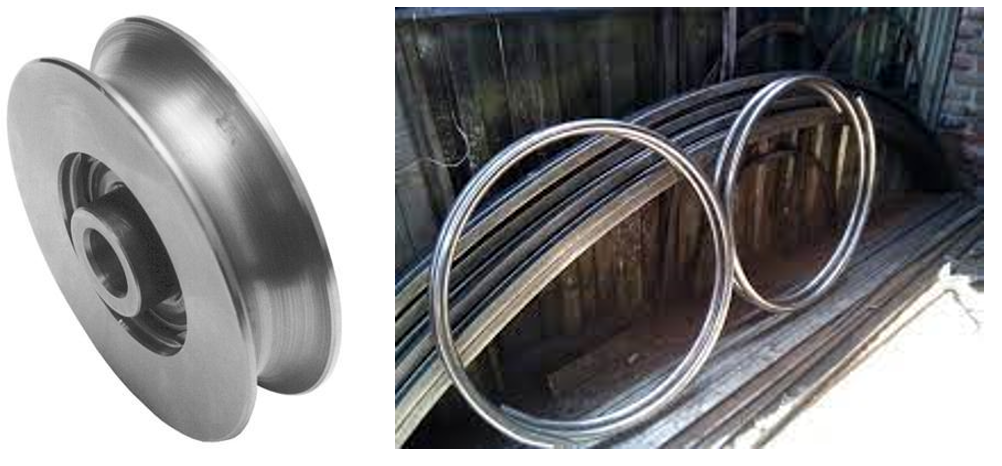
\includegraphics[width=\columnwidth]{imagenes/ruedaRielPistaCircular.PNG}
	\caption{Geometría de una rueda tipo riel (izquierda) y un perfil circular rolado (derecha).}
	\label{fig:rueda_pista}
\end{figure}

% \textbf{Trabajo Terminal II}
% 	\item Fabricar e implementar los sistemas diseñados mediante manufactura, compra, impresión o ensamble de componentes para su posterior verificación de funcionamiento.
% 	\item Integrar los sistemas construidos mediante adaptación y sintonización que permita lograr una afinidad y sinergia entre ellos, para verificar y validar su funcionamiento en conjunto.
% 	\item Verificar el correcto funcionamiento de los sistemas construidos a través de pruebas y mediciones, con el fin de validar el cumplimiento de los requerimientos establecidos en la fase de diseño.
% 	\item Ajustar y acondicionar los parámetros necesarios que permitan el ensamble de todos los sistemas, para asegurar el adecuado funcionamiento del seguidor solar.




%%%%%%fin del archivo
\endinput 